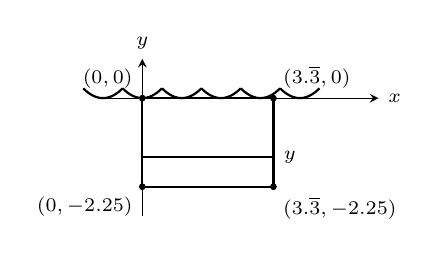
\begin{tikzpicture}[x=.5cm,y=.5cm,>=stealth]
\draw[thick] (0,0) -- (3.33,0) --  (3.33,-2.25) -- (0,-2.25) --cycle;

\draw [fill=black] 	(3.33,0) circle (1pt) node [above right] {\scriptsize $(3.\overline{3},0)$}
										(3.33,-2.25)circle (1pt) node [below right] {\scriptsize $(3.\overline{3},-2.25)$}
										(0,-2.25)circle (1pt) node [below left] {\scriptsize $(0,-2.25)$};
										\draw [fill=black] 	(0,0) circle (1pt) node [above left] {\scriptsize $(0,0)$};
										
\draw [{\colortwo},thick]  (0,-1.5) -- (3.33,-1.5) node [right,black] {\scriptsize $y$};
%										
\draw [->] (0,-3) -- (0,1) node [above] {\scriptsize $y$};
\draw [->] (-1,0) -- (6,0) node [right] {\scriptsize $x$};
%
%\foreach \x in {-2,-1,1,2}
%{
%	\draw (\x,10.2) -- (\x,9.8) node [below] {\scriptsize $\x$};
%}
%
%\foreach \x in {-10,-8,-4,-2}
%{
%	\draw (.2,{\x+10}) -- (-.2,{\x+10}) node [left] {\scriptsize $\x$};
%}
%
\foreach \x in {-1,0,1,2,3,4}
{%
		\begin{scope}[shift={(\x*1,0)}]		
		\draw [{\colorone},thick] (-.5,.25) parabola bend (0,0) (.5,.25);
		\end{scope}
}
%
%\draw (7,1) node {\scriptsize water line};

%\draw (4.3,3) -- (4.7,3)
%			(4.3,10) -- (4.7,10)
%			(4.5,3) -- node [pos=.5,rotate=-90,above] {\scriptsize $d(y) = -y$} (4.5,10);


\end{tikzpicture}

